\documentclass[12pt]{article}
\usepackage[utf8]{inputenc}
\usepackage[T1]{fontenc}
\usepackage[spanish]{babel}
\usepackage{amsmath, amssymb}
\usepackage{geometry}
\usepackage{listings}
\usepackage{color}
\usepackage{graphicx}
\usepackage{hyperref}
\usepackage{fancyhdr}
\geometry{a4paper, margin=2.5cm}
\usepackage{lmodern}
\usepackage{float}

\begin{document}
	
	% Portada estilo personalizado
	\begin{titlepage}
		\centering
		\vspace*{2cm}
		
		{\LARGE\textbf{Tarea \#3 \\
		Algoritmos de búsqueda en texto}}\\[0.3cm]
		
		\textit{Algoritmos y Estructuras de Avanzadas/ Magíster en Ciencias de la Computación}\\
		\textit{Departamento Ciencias de la Computación y}\\
		\textit{Tecnologías de la Información}\\[0.5cm]
		
		{\large\textbf{Universidad del Bío-Bío}}\\[2cm]
		
		\begin{flushleft}
			\textbf{Profesor:} Gilberto Gutiérrez
		\end{flushleft}
		
		\begin{flushright}
			Diego Arteaga \\
			Rodrigo Sandoval
		\end{flushright}
		
		\vfill
		\textbf{Otoño 2025}
	\end{titlepage}
	
	% Inicio del contenido del informe
	\section{Introducción}
	
	\section{Implementación de algoritmos de búsqueda}
	En la presente sección se muestra como se implemento y como se compara el rendimiento de ejecución de los algoritmos de búsqueda en texto \texttt{KMP} y \texttt{RABIN-KARP}, para los cuales se tuvieron las siguientes consideraciones previas.
	
	\begin{description}
		\item Un alfabeto $\sum$ \{0,1,2,3,4,5,6,7,8,9\}.
		\item Casos en que el texto (T) tenga diferentes largos.
		\item Casos en que el patrón (P) tenga diferentes largos.
	\end{description}
	
	\subsection{Algoritmo KMP}
	Para la implementación del algoritmo \texttt{KMP} se utiliza una función de pre-procesamiento denominada \texttt{computeLPS}, la cual construye la tabla de prefijos-sufijos más largos (LPS).
	
	El algoritmo presenta una complejidad O(n+m) en el peor caso, por lo cual es de un carácter eficiente para patrones largos y textos grandes. De igual manera, presenta un mejor funcionamiento en patrones con alta repetición.
	
	A continuación se presenta el algoritmo \texttt{KMP} implementado.
	
	\begin{figure}[H]
		\centering
		\includegraphics[width=0.8\textwidth]{KMP.png}
		\caption{Implementación KMP}
		\label{fig: Algoritmo KMP}
	\end{figure}
	
	A continuación se presentan los tiempos de ejecución del algoritmo \texttt{KMP}  tanto con un patrón de tamaño fijo (5) y un texto variables, como un texto fijo (100.000) y un patrón variable.
	
	\begin{table}[H]
		\centering
		\begin{tabular}{|c|c|}
			\hline
			\textbf{Tamaño Texto} & \textbf{KMP (ns)} \\
			\hline
			1000     & 147080   \\
			10000    & 651180   \\
			50000    & 1049900  \\
			100000   & 610380   \\
			500000   & 3249730  \\
			1000000  & 6435360  \\
			\hline
		\end{tabular}
		\caption{Tiempos de ejecución del algoritmo \texttt{KMP} con texto variable y patrón de tamaño 5}
		\label{tab:kmp}
	\end{table}
	
	\begin{table}[H]
		\centering
		\begin{tabular}{|c|c|}
			\hline
			\textbf{Tamaño Patrón} & \textbf{KMP (ns)} \\
			\hline
			2     & 711810  \\
			5     & 756330  \\
			10    & 881170  \\
			20    & 672370  \\
			50    & 679420  \\
			100   & 765440  \\
			200   & 648120  \\
			500   & 647670  \\
			1000  & 663190  \\
			\hline
		\end{tabular}
		\caption{Tiempos de ejecución del algoritmo \texttt{KMP} con texto fijo (100.000) y patrón variable}
		\label{tab:kmp_patron}
	\end{table}
	
	
	\subsection{Algoritmo Rabin-Karp}
	
	Para la implementación del algoritmo \texttt{Rabin-Karp} se utilizo un hashing rodante que permite comparar eficientemente subcadenas, ademas de considerar una base numérica de 10, apta para dígitos del 0 al 9, así mismo, un número primo de 101 para reducir colisiones. 
	
	El algoritmo posee una complejidad promedio de O(n+m), con un peor caso de O(nm), por lo cual es muy eficiente para patrones pequeños y para la detección de múltiples patrones.
	
	A continuación se presenta el algoritmo \texttt{Rabin-Karp} implementado.
	
	\begin{figure}[H]
		\centering
		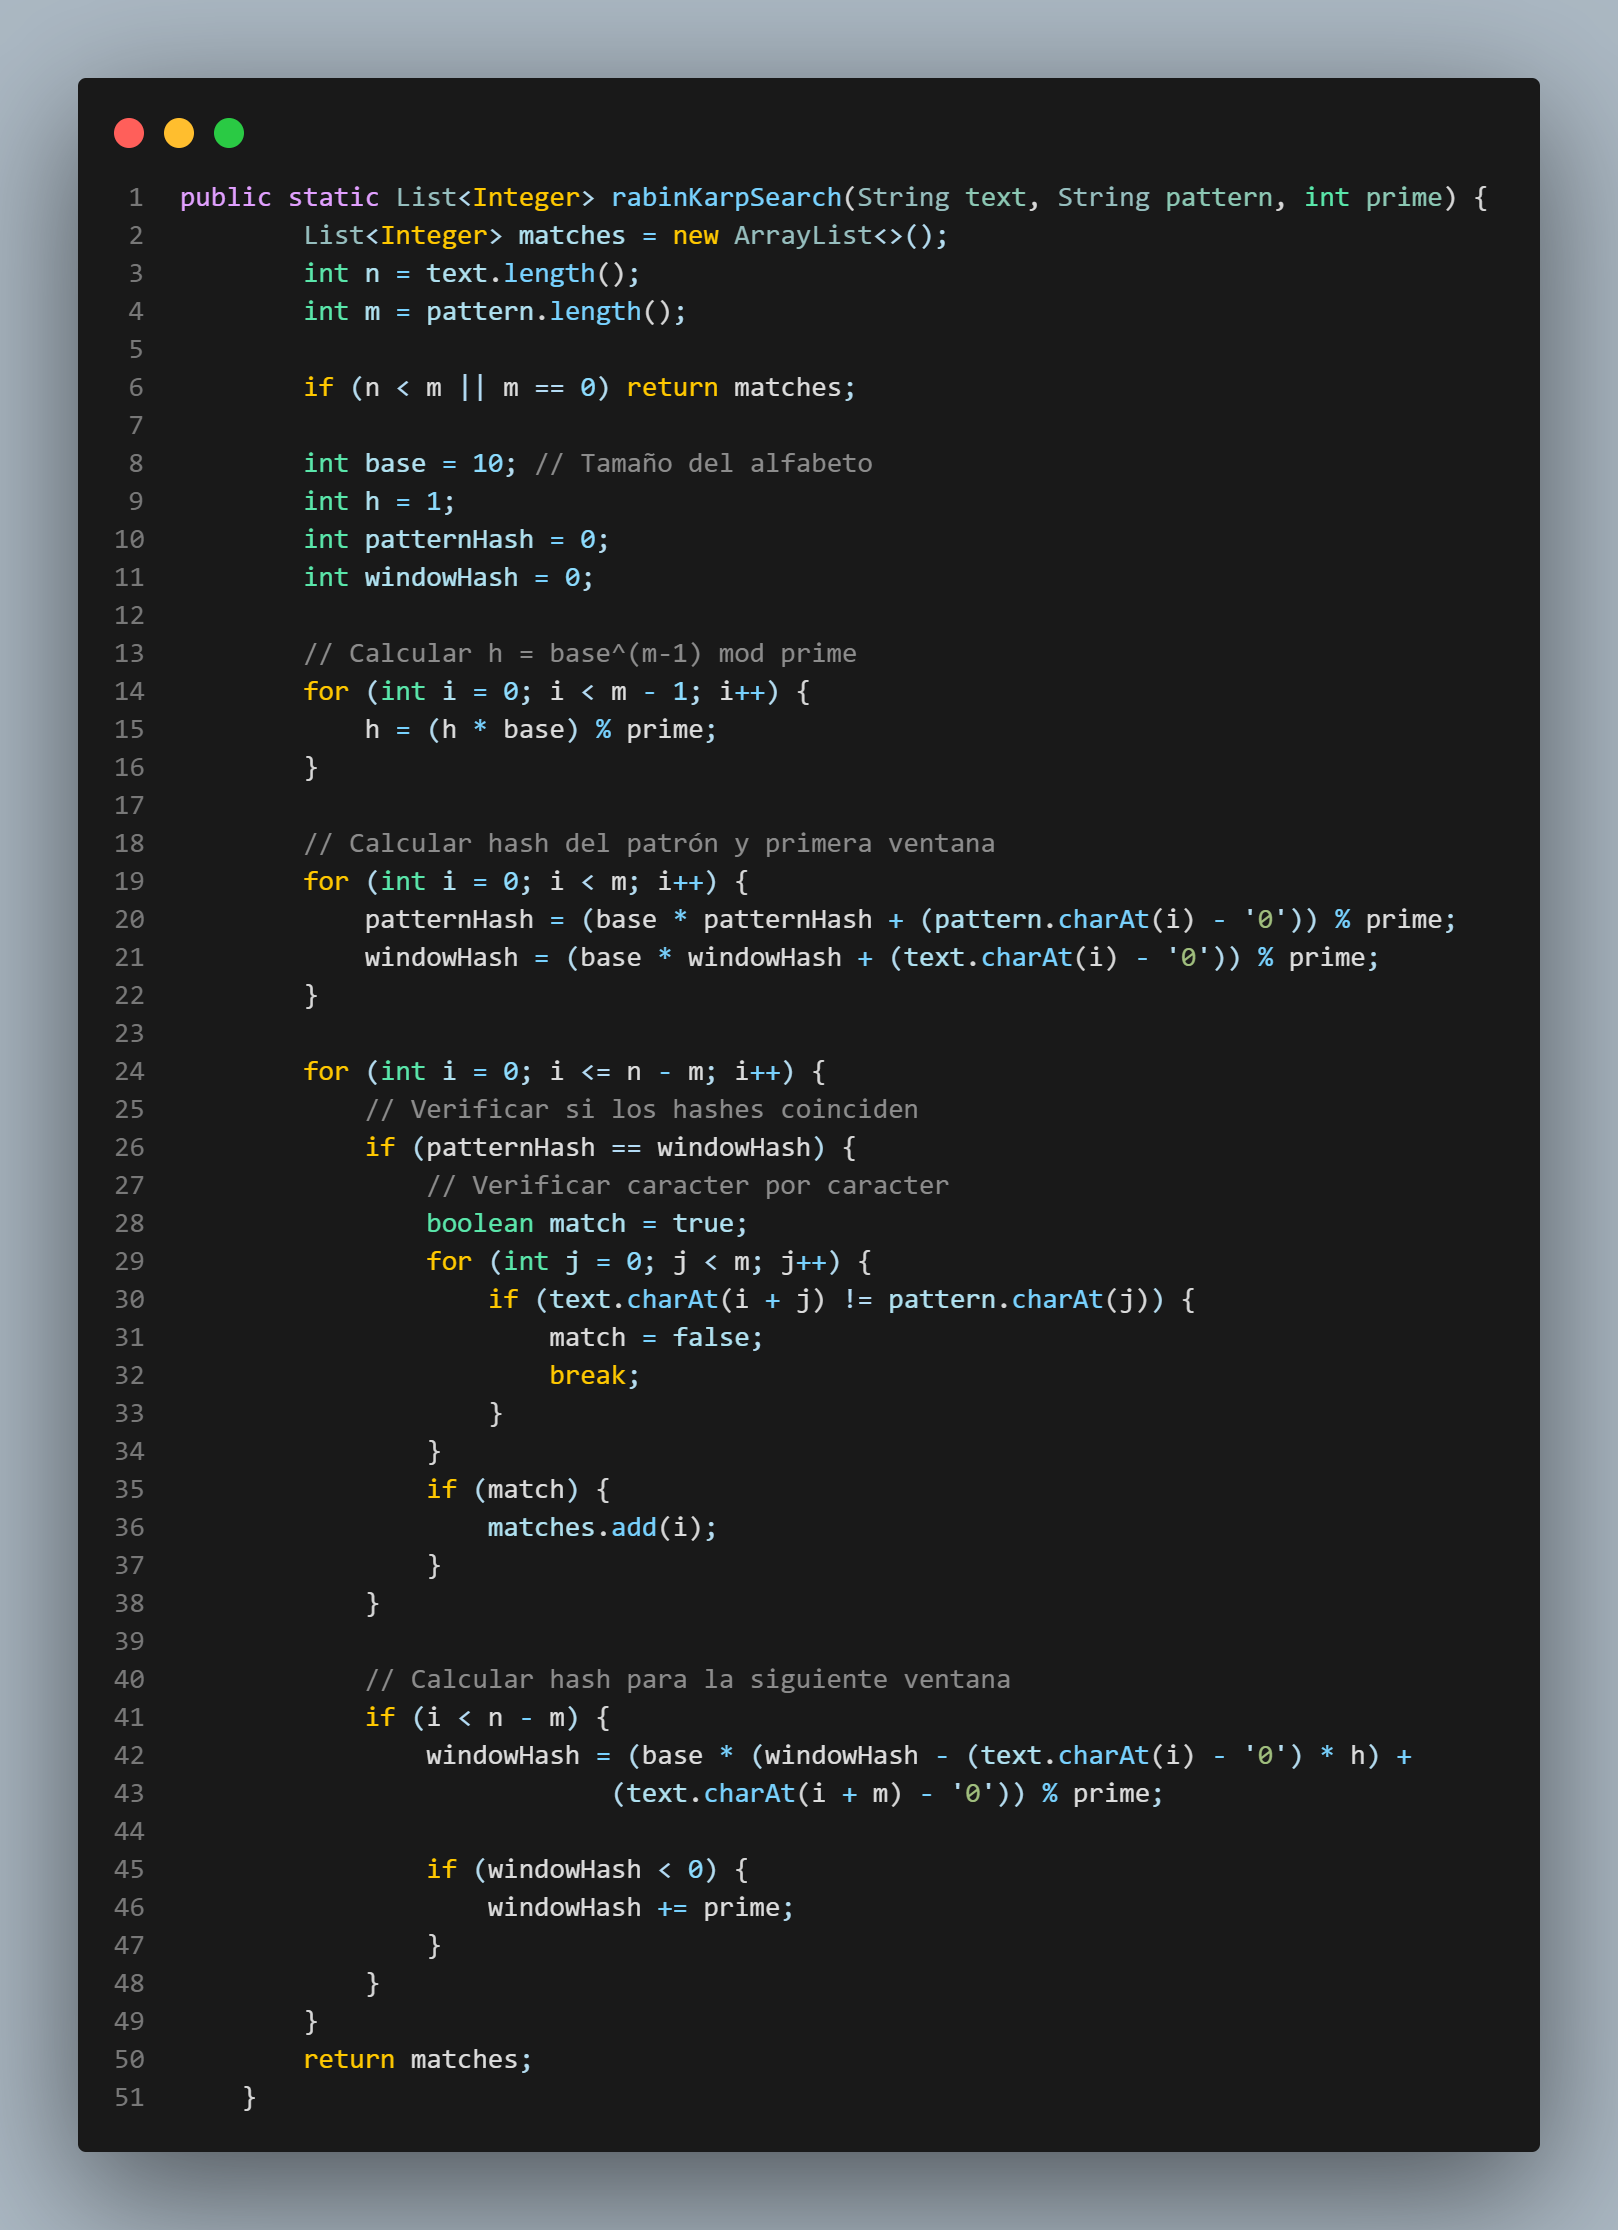
\includegraphics[width=0.8\textwidth]{RK.png}
		\caption{Implementación Rabin-Karp}
		\label{fig: Algoritmo Rabin-Karp}
	\end{figure}
	
	A continuación se presentan los tiempos de ejecución del algoritmo \texttt{Rabin-Karp}  tanto con un patrón de tamaño fijo (5) y un texto variables, como un texto fijo (100.000) y un patrón variable.
	
		\begin{table}[H]
		\centering
		\begin{tabular}{|c|c|}
			\hline
			\textbf{Tamaño Texto} & \textbf{Rabin-Karp (ns)} \\
			\hline
			1000     & 118310   \\
			10000    & 613050   \\
			50000    & 1321960  \\
			100000   & 678410   \\
			500000   & 3486370  \\
			1000000  & 7104310  \\
			\hline
		\end{tabular}
		\caption{Tiempos de ejecución del algoritmo \texttt{Rabin-Karp} con texto variable y patrón de tamaño 5}
		\label{tab:Rabin-Karp}
	\end{table}
	
	\begin{table}[H]
		\centering
		\begin{tabular}{|c|c|}
			\hline
			\textbf{Tamaño Patrón} & \textbf{Rabin-Karp (ns)} \\
			\hline
			2     & 668720  \\
			5     & 716260  \\
			10    & 1429650  \\
			20    & 855830  \\
			50    & 1351530  \\
			100   & 858680  \\
			200   & 837580  \\
			500   & 832910  \\
			1000  & 851460  \\
			\hline
		\end{tabular}
		\caption{Tiempos de ejecución del algoritmo \texttt{Rabin-Karp} con texto fijo (100.000) y patrón variable}
		\label{tab:Rabin-Karp_patron}
	\end{table}
	
	Durante el apartado de resultados experimentales \ref{resultados_experimentales} se llevará a cabo una comparativa de ambos algoritmos.
	
	\section{Descripción del algoritmo}
	
	\section{Resultados experimentales}
	\label{resultados_experimentales}\textbf{}
	
	En esta sección se comparara el rendimiento de los algoritmos \texttt{KMP} y \texttt{Rabin-Karp}, para los cuales se responderán las siguientes preguntas:
	
	\begin{description}
		\item[i] Que ocurre si varía el largo del texto manteniendo fijo el tamaño del patrón: ¿Cual presenta mejor rendimiento?.
		\item[ii] Que pasa si se mantiene fijo el tamaño del texto y se varía el tamaño del patrón.
	\end{description}
	
	\begin{table}[H]
		\centering
		\resizebox{\textwidth}{!}{
			\begin{tabular}{|c|c|c||c|c|c|}
				\hline
				\multicolumn{3}{|c||}{\textbf{Escenario 1: Texto variable, patrón fijo (tamaño 5)}} & \multicolumn{3}{c|}{\textbf{Escenario 2: Texto fijo (100,000), patrón variable}} \\
				\hline
				\textbf{Tamaño Texto} & \textbf{KMP (ns)} & \textbf{Rabin-Karp (ns)} & \textbf{Tamaño Patrón} & \textbf{KMP (ns)} & \textbf{Rabin-Karp (ns)} \\
				\hline
				1000 & 147080 & 118310 & 2 & 711810 & 668720 \\
				10000 & 651180 & 613050 & 5 & 756330 & 716260 \\
				50000 & 1049900 & 1321960 & 10 & 881170 & 1429650 \\
				100000 & 610380 & 678410 & 20 & 672370 & 855830 \\
				500000 & 3249730 & 3486370 & 50 & 679420 & 1351530 \\
				1000000 & 6435360 & 7104310 & 100 & 765440 & 858680 \\
				& & & 200 & 648120 & 837580 \\
				& & & 500 & 647670 & 832910 \\
				& & & 1000 & 663190 & 851460 \\
				\hline
			\end{tabular}
		}
		\caption{Tiempos de ejecución de los algoritmos KMP y Rabin-Karp para dos escenarios distintos.}
		\label{tab:algoritmos_KMP_Rabin-Karp}
	\end{table}
	
	Para el escenario 1 se puede considerar que en textos pequeños entre mil y diez mil, \texttt{Rabin-Karp} es más rápido, ya que presenta un menor tiempo de ejecución. A partir de los cincuenta mil caracteres, \texttt{KMP} presenta una superación a \texttt{Rabin-Karp}, finalmente con textos muy grandes entre quinientos mil y un millón, \texttt{KMP} mantiene una ventaja.
	
	Para el escenario 2 se puede indicar que \texttt{KMP} es consistentemente más rápido que \texttt{Rabin-Karp} cuando el patrón crece. Por otro lado, \textbf{Rabin-Karp} empeora significativamente con patrones más grandes, esto para diez, cincuenta y 100 caracteres. Sin embargo, \texttt{KMP} mantiene un tiempo estable, independientemente del tamaño del patrón.
	
	En respuesta a la pregunta \texttt{i} se puede indicar que para textos pequeños entre mil y diez mil, \textbf{Rabin-Karp} es más eficiente, mientras que para textos mas grandes entre cincuenta mil y un millón, \texttt{KMP} es más rápido. Con esto se puede indicar que \texttt{Rabin-Karp} es óptimo apra búsquedas con patrones cortos de texto y no muy extensos.
	
	En respuesta a la pregunta \texttt{ii} se puede indicar que \texttt{KMP} siempre es más eficiente, especialmente con patrones grandes. Mientras que \texttt{Rabin-Karp} empeora cuando el patrón crece, debido a la sobrecarga del hash rodante. Por lo cual es posible indicar que \texttt{KMP} es la mejor opción si el patron varía en tamaño.
	
	\section{Conclusiones}
	
	\section{Anexos}
	\subsection{Código implementado}
	\href{URL}{GitHub}
	
\end{document}





















